    The DUNE implementation runs on a BeagleBone Black Industrial (BBB), pictured in figure \ref{fig:bbb}. A cape is connected to the BeagleBone, in turn connected to both a GNSS receiver, and a Pixhawk 2.1 (also called The Cube flight controller). The Pixhawk has another GNSS receiver and a magnetometer connected to it. The full payload sits conveniently in a peli case. A simple block diagram illustrates this in figure \ref{fig:hardware-connection-diagram}\\
    
    \begin{figure}
        \centering
        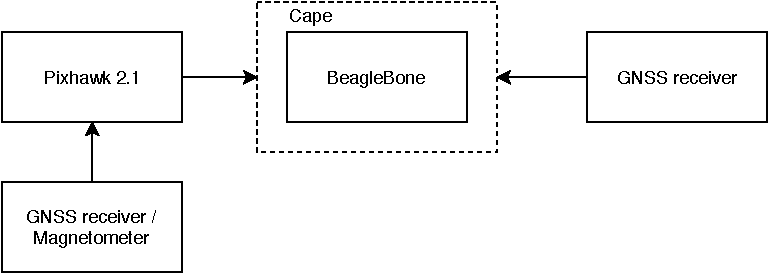
\includegraphics{Implementation/Images/hardware-schematic.pdf}
        \caption{Block diagram of the hardware package}
        \label{fig:hardware-connection-diagram}
    \end{figure}
    
    \subsubsection{BeagleBone}
    %BBB
    The BeagleBone Black is a powerful embedded computer board capable of running several different operating systems, such as Ubuntu. It contains both USB, HDMI mini and Ethernet ports, as well as pin headers with both UART, SPI and I2C. By default the BeagleBone comes with a stripped down linux distribution called Angstrom, but it has been flashed with the Glued linux distribution through the onboard SD-card. The BeagleBone can be controlled by SSH over the ethernet port, where the user can start or stop processes, modify configuration files or transfer data to or from the BeagleBone. The router in the case provides the user with additional ethernet ports and a DHCP server to simplify the connection process.\\
    
    \todo{fix figure BBB}
    \begin{figure}
        \centering
        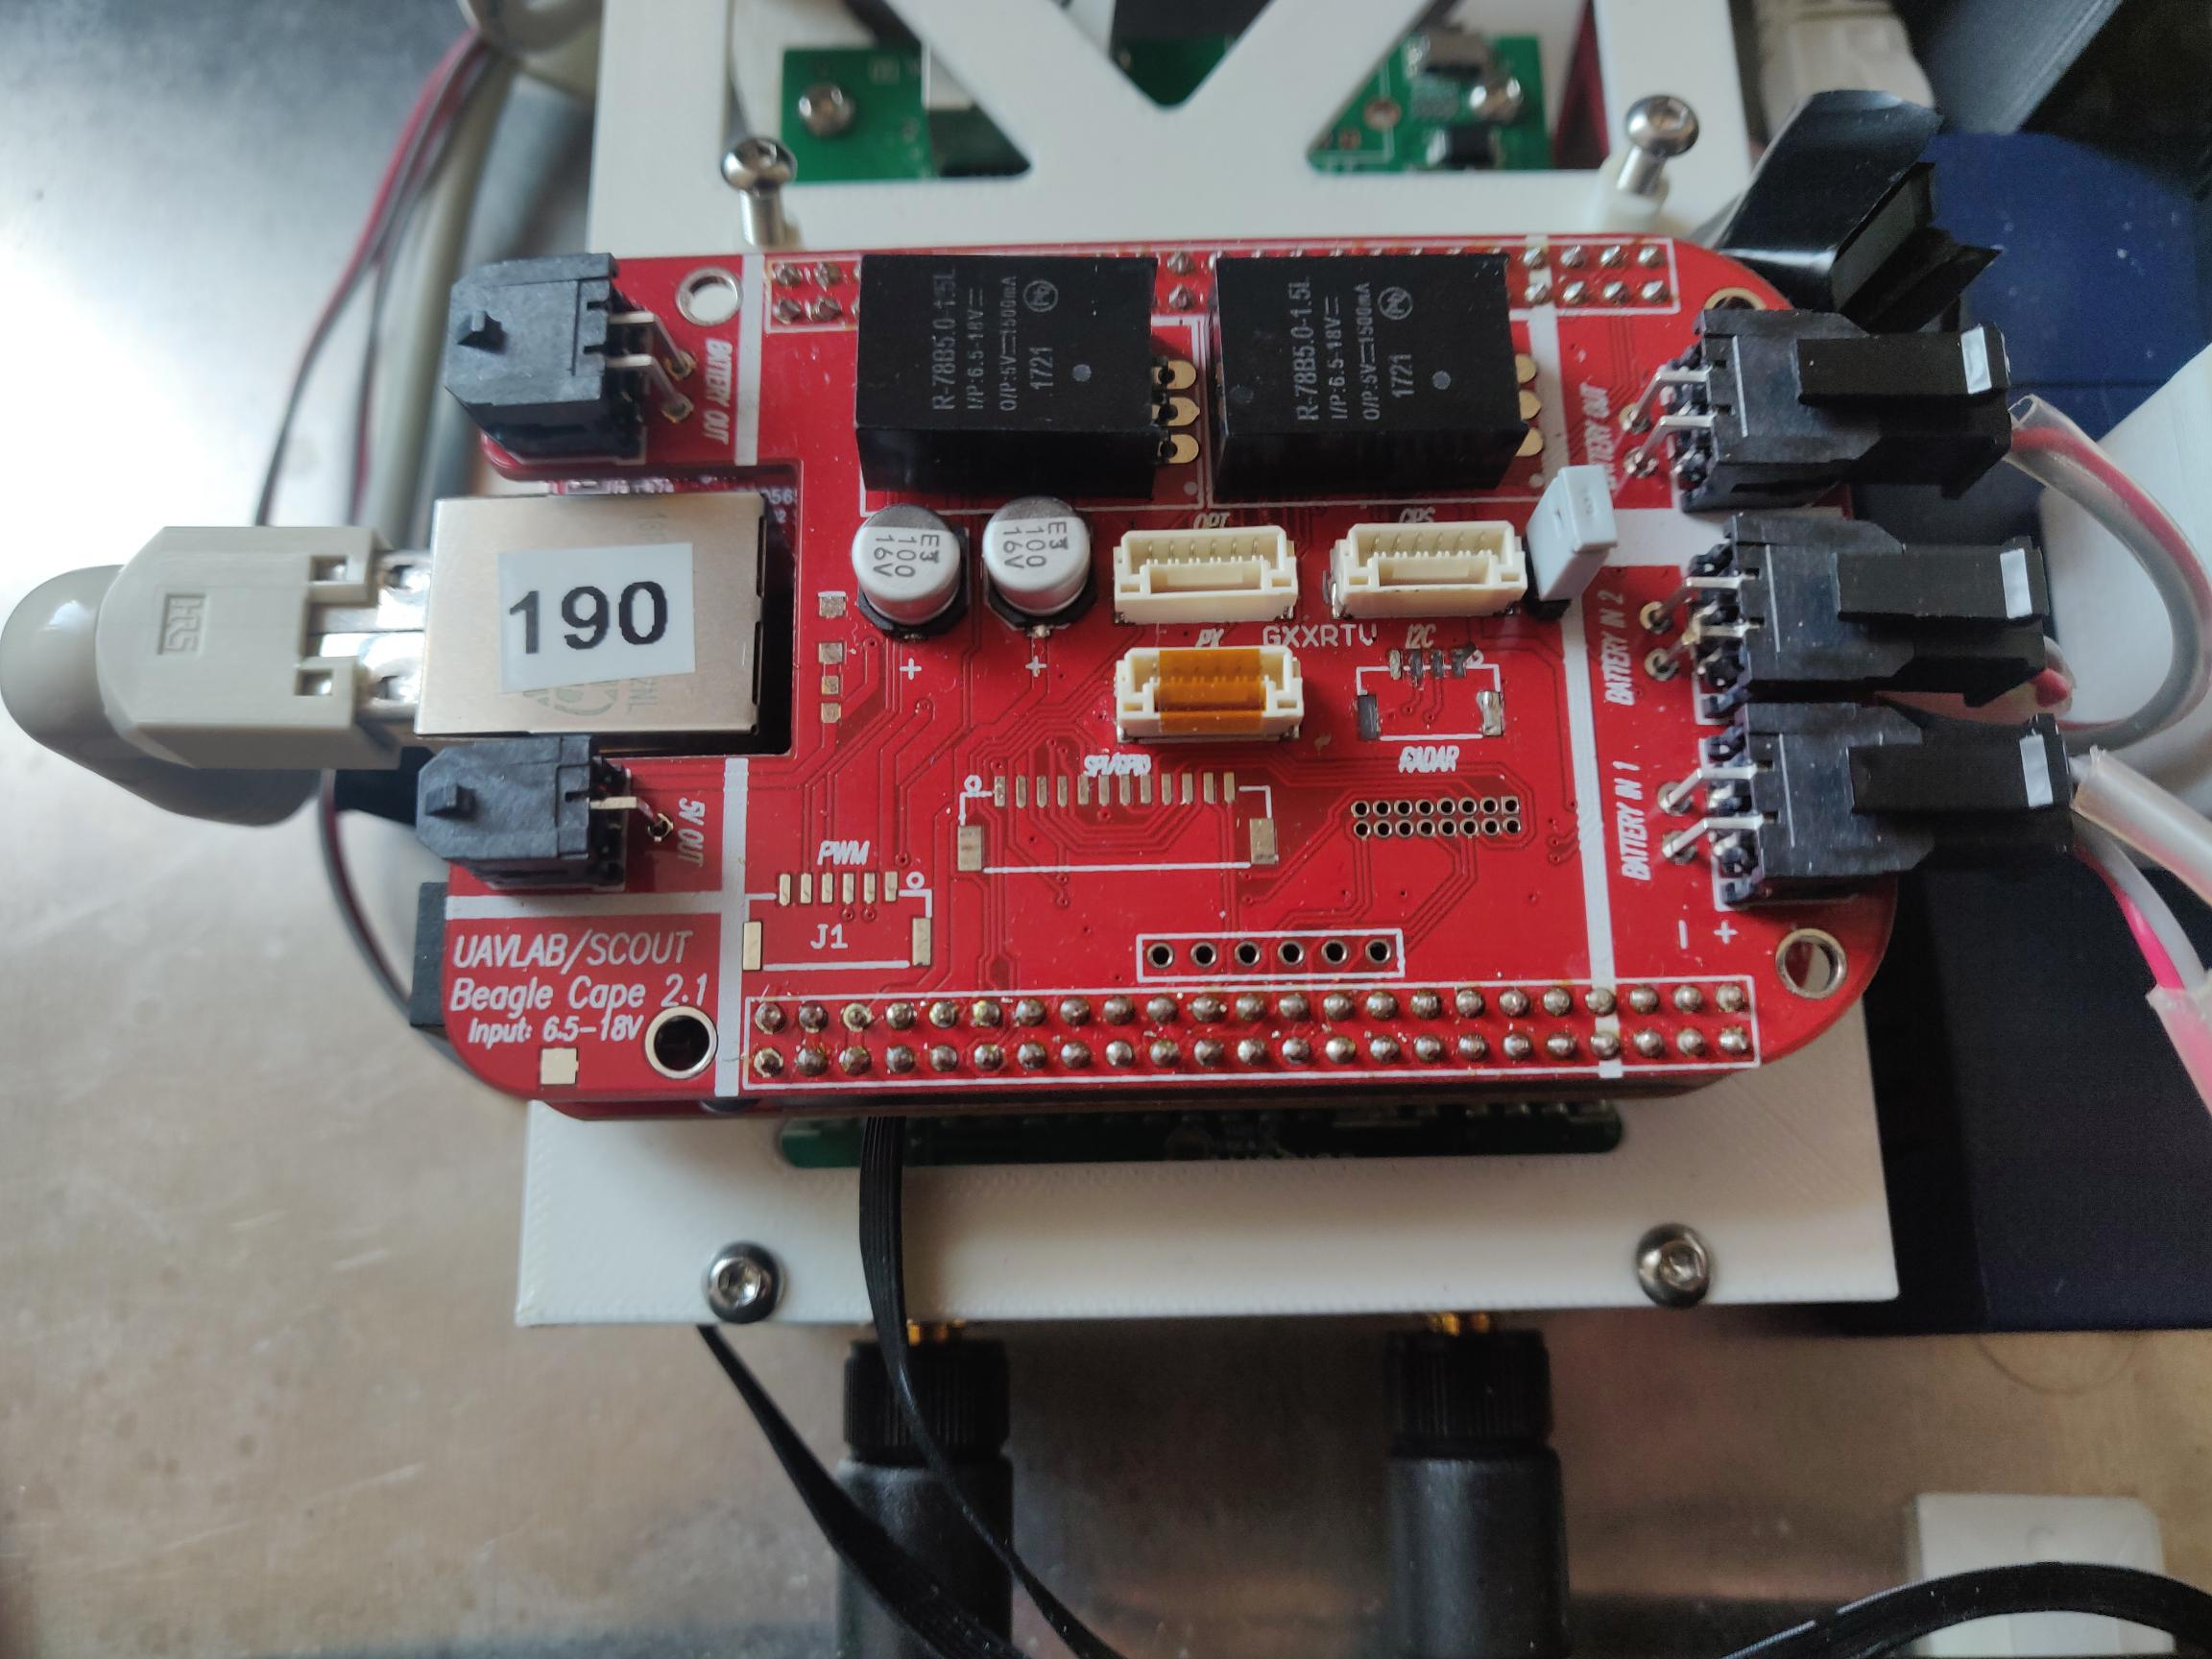
\includegraphics[scale=0.1]{Implementation/Images/BBB.jpg}
        \caption{A beaglebone with a cape (midlertidig)}
        \label{fig:bbb}
    \end{figure}
    
    %Cape
    The cape is a design of the UAVlab at NTNU and was soldered by hand. There are several reasons for including this in the payload. Firstly, it contains connector ports for a GNSS receiver, a pixhawk, two SPI ports, an I2C port and a PWM port, greatly reducing clutter from cables. Secondly, it also contains four molex power connectors, two for voltage input and two for voltage output. It can therefore be used as a power hub for the whole system. Both the pixhawk, receiver and even the ethernet router. Since there are two voltage inputs, power sources can also be \textit{hot-swapped}, keeping the system from powering down. This is convenient when switching batteries or for keeping the BeagleBone running in post-processing. Another useful feature of the cape is its real time clock, powered by a backup battery. With this, the BeagleBone will keep track of time even when turned off, which is especially important for logging purposes as logs are automatically named according to date and time and a name conflict will result in the original log being overwritten. Without the real time clock, the logs would usually be overwritten during startup as all would be named with respect to the BeagleBone's default epoch.\\
    
    \subsubsection{Sensors}
    %Receiver
    The GNSS receiver connected to the BeagleBone is an UBlox NEO-M8T mounted on an InCase series NEO-M8T board. The LEA-M8T breakout board was also used for early testing on a computer as it comes with a built in USB port, but the two receivers are otherwise much the same. Both support GPS, GLONASS, BeiDou and Galileo, as well as the QZSS and SBAS augmentation systems \cite{ublox:neo-m8t}. The receiver uses a Tallysman TW4421-00 Wideband Dual Feed antenna.\\
    \todo{fix figure neo-m8t}
    \begin{figure}[!htbp]
        \centering
        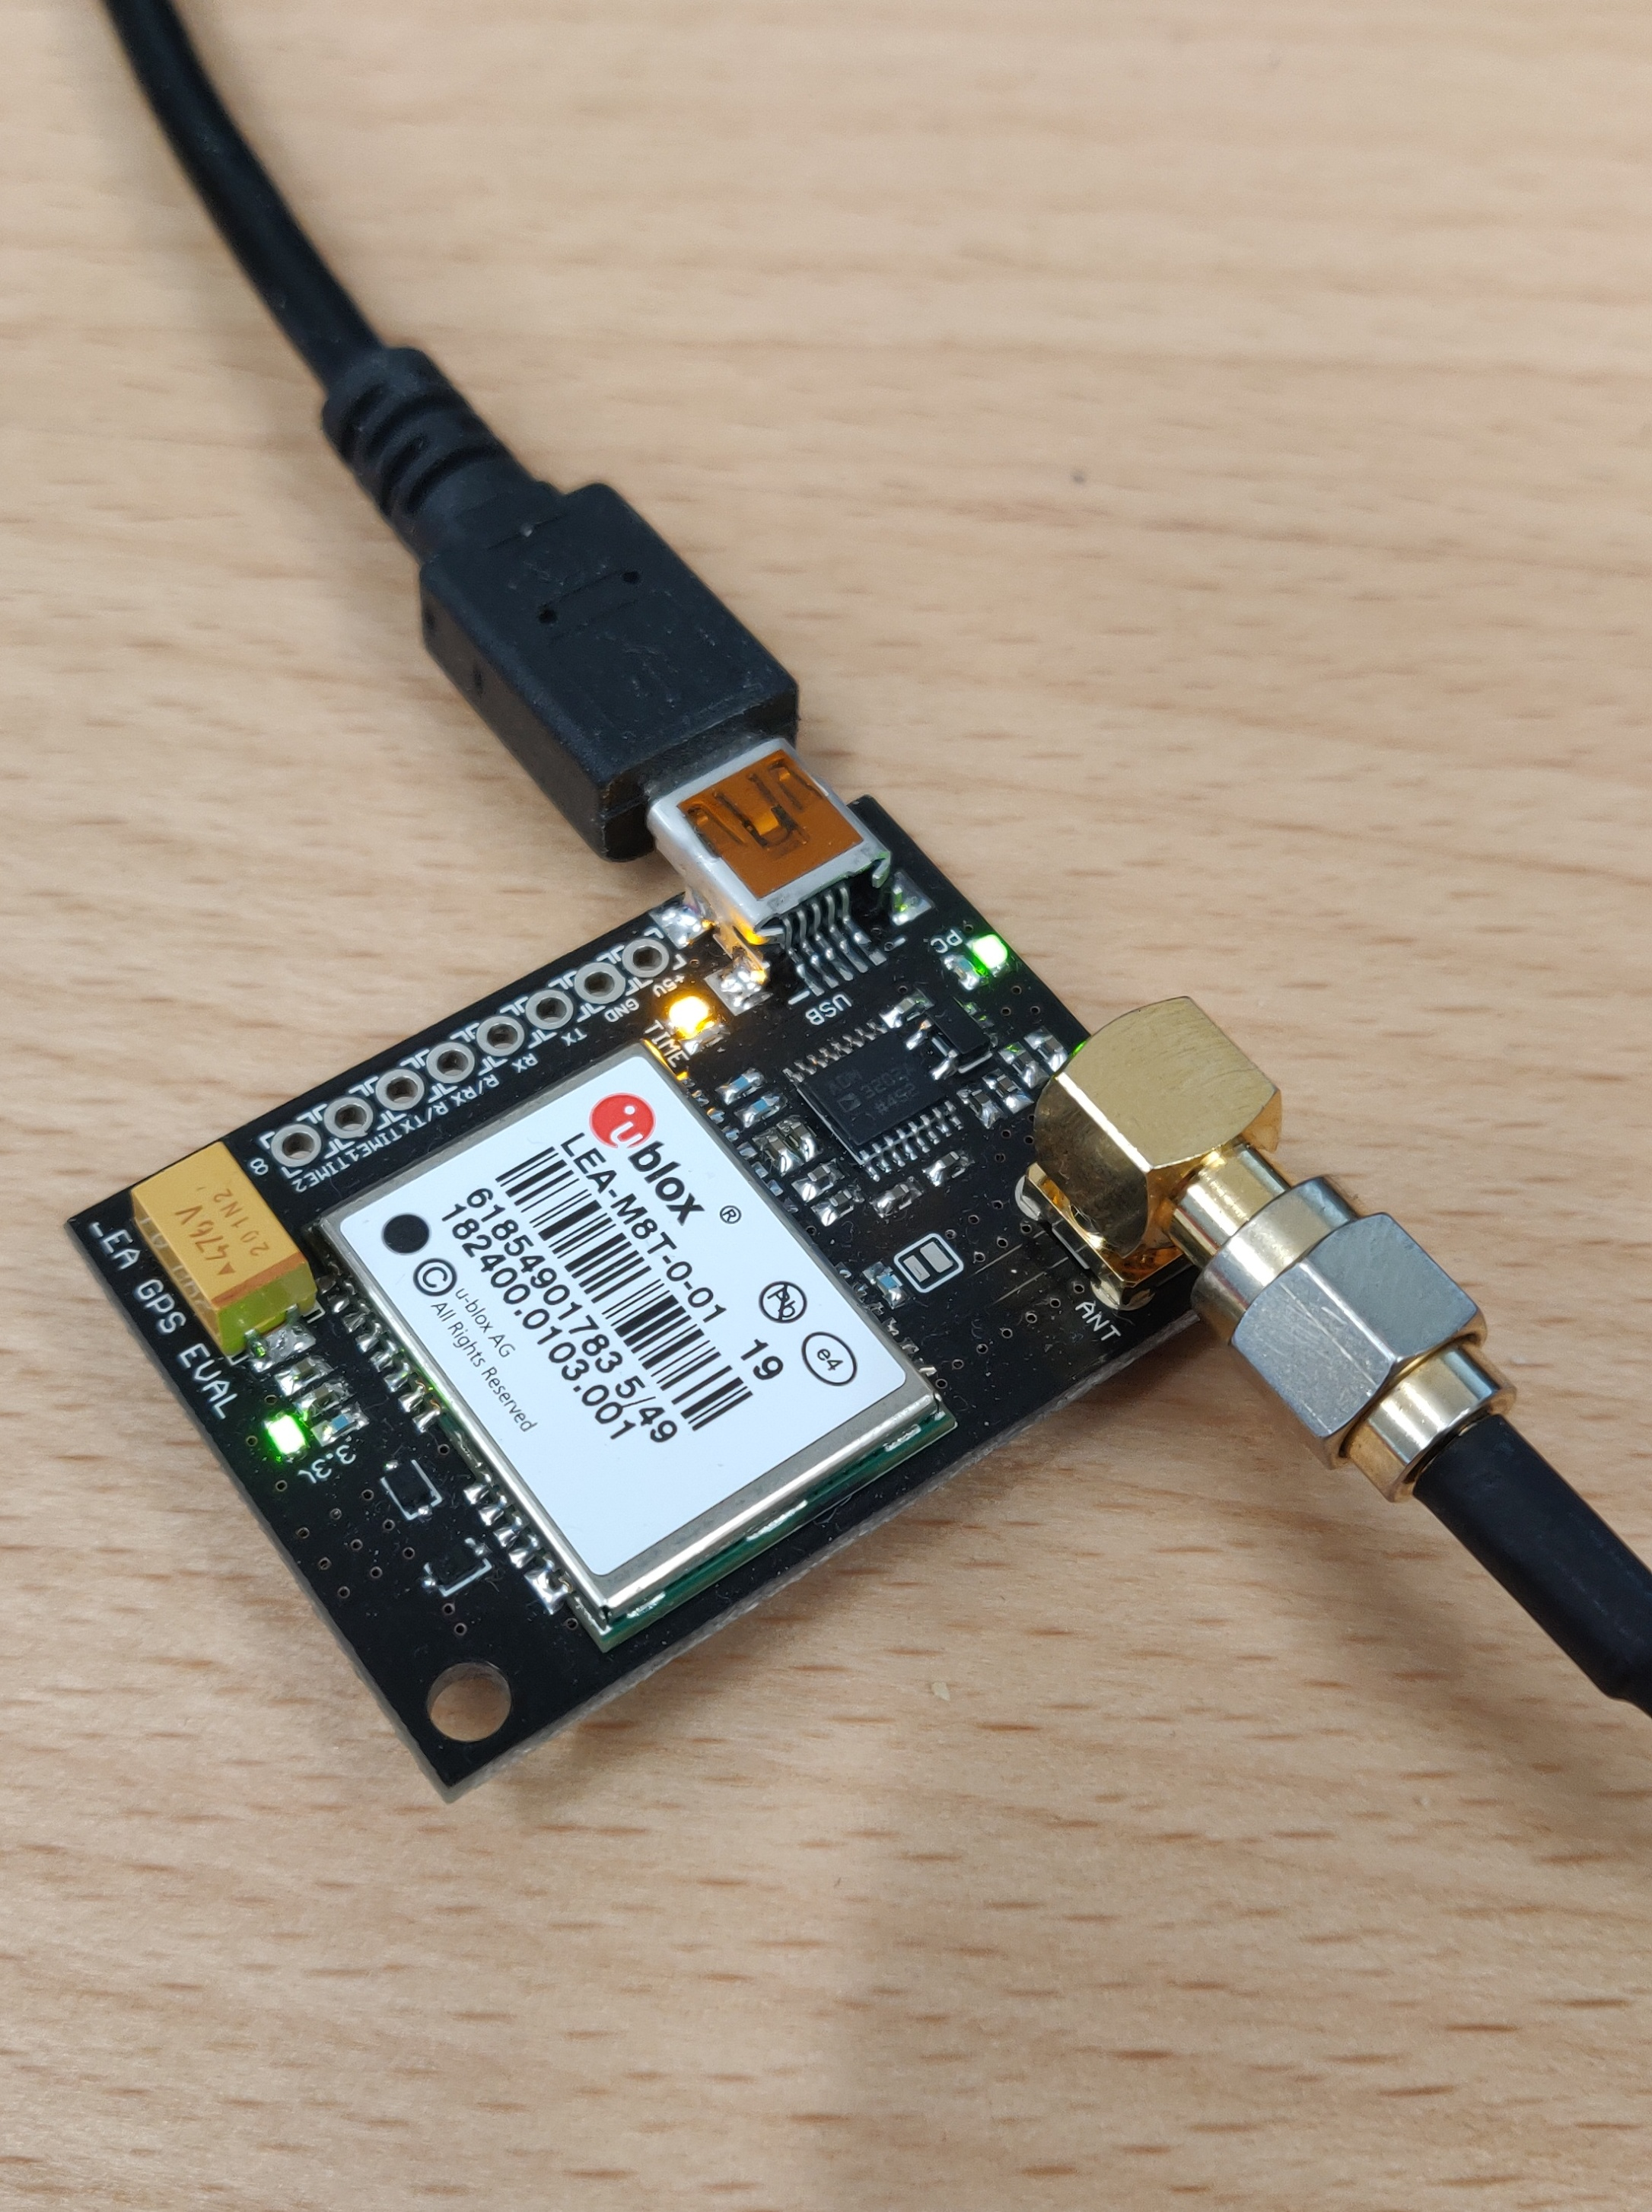
\includegraphics[angle=180, scale=0.05]{Implementation/Images/lea-m8t.jpg}
        \caption{A NEO-M8T receiver (midlertidig)}
        \label{fig:neo-m8t}
    \end{figure}
             
    %PixHawk
    Imu measurements are read from the pixhawk flight controller. It contains three separate nine-axis IMU's (3-axis gyroscope, accelerometer and magnetometer) for redundancy, two of which are mechanically vibration-isolated. Additionally, an external GPS and magnetometer is connected. It runs the ArduPlane flight stack and keeps an internal state estimate that is dispatched to the DUNE system, as explained in section \ref{sec:imp:ekf-dune}. 
    %\begin{figure}
    %    \centering
    %    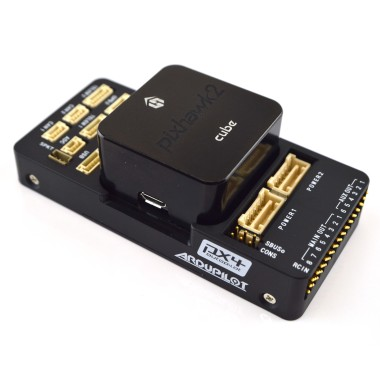
\includegraphics[scale=0.6]{Implementation/Images/pixhawk-cube.jpg}
    %    \caption{The pixhawk 2.1, The Cube}
    %    \label{fig:px-cube}
    %\end{figure}
    
    %Ground station
    
    %Router?
    \missingfigure[]{Full system}
    %Lea-m8t (mention config) with antenna, pixhawk (imu), BBB with glued and dune, Peli case? (probably not), separate BBB with receiver running rtklib-rtkrcv and str2str for post processing (ground truth)
    
%\subsection{Glued configuration}
%    \label{sec:imp:glued-conf}
    \todo{Describe glued config?}

% \cite{zolich2015unmanned}

%Receiver
% Configuring the receiver
% U-center to configure messages
% rtklib cmd-file
% chosen ubx messages, nmea messages